% ======================================================================================
%  The Camera, the Split, and the Label — body (three-check audit of GRAPE progression benchmarks)
% ======================================================================================

\begin{abstract}
On the public GRAPE benchmark, deep networks report glaucoma-progression AUCs as high as \num{0.96}. We audit the
benchmark's published record and find that, at this sample size, none of the reported numbers can be distinguished from
a trivial baseline. We re-evaluate all five published models under one fixed protocol of three checks: a device-only baseline
(on GRAPE, the acquisition camera), a patient-grouped split, and a test that the input is disjoint from the window that
defines the label. As a positive test, we predict the shipped label from the baseline visit, before its trend is
computable. Image features from a frozen fundus model identify the camera at AUC \num{0.98}--\num{1.00}, the camera alone predicts
progression at \num{0.56}--\num{0.60}, and a device-controlled fundus model does no better. Under a fair,
device-controlled evaluation every reported number is no better than it, and
one model's own released code falls from \num{0.87}/\num{0.96}/\num{0.92} to \num{0.43}/\num{0.54}/\num{0.55}
(PLR2/PLR3/MD). The label
is a trend fit to the visual-field series, and we introduce a circularity dial that measures how it is recovered from
those defining statistics, with no image, as the input window approaches the window that defines it (AUC \num{0.90}).
The checks need only metadata GRAPE already includes: a device label, patient identifiers, the label's definition, and
visit dates. We release a fixed split and a reporting template so the audit can be reused.
\end{abstract}

% ======================================================================================
\section{Introduction}
\label{sec:intro}

Glaucoma is the leading cause of irreversible blindness \citep{tham2014global}, and its management depends on
progression, the question of whether an eye is worsening fast enough to change treatment. The public GRAPE benchmark
\citep{huang2023grape} made this a machine-learning task, pairing fundus photographs and visual-field tests with
follow-up. Recent models report strong results: a single baseline color fundus photograph (CFP) reaches AUC
\num{0.71}--\num{0.80} \citep{huang2023grape}, models that read a sequence of photographs reach \num{0.96} (TSDF
\citep{song2025tsdf}) and \num{0.88} (DiffSight-Former \citep{huang2026diffsight}), and a model that fuses the visual field with fundus reaches \num{0.849}
\citep{zheng2025gppm}.

Whether these numbers reflect the eye or the way the data were collected is a question about evaluation, not the model.
A single held-out AUC can be high for reasons that have nothing to do with disease. A model can read the
acquisition camera instead of the retina \citep{geirhos2020, badgeley2019confound, degrave2021}. One patient's two eyes
can leak across the train and test split \citep{tampu2022leakage, kapoor2023leakage}. The input can already contain the
measurements that define the label. None of these is visible in a single number. The target is contested too: standard
visual-field progression algorithms agree on as little as \num{2.5}\% of eyes \citep{saeedi2019}, so even a perfect
model chases a moving definition.

We turn these concerns into a compact, reusable audit and apply it to GRAPE and all five published models
(Fig.~\ref{fig:audit}). Two kinds of evidence stay separate: the shortcuts, which use no outcome labels and hold on the
well-powered endpoints, and the recovered progression signal, which rests on \num{14} to \num{40} events
\citep{riley2020samplesize} and so is read as an interval.

\paragraph{Contributions.}
\begin{itemize}[leftmargin=1.2em, itemsep=1pt, topsep=1pt]
\item \textbf{The first audit of this benchmark's whole published record} (\S\ref{sec:audit}, Fig.~\ref{fig:audit}).
  Three checks control shortcuts that can produce a high AUC (a device floor, a fair split, and a circularity check), and a
  forecast from an early visit supplies the positive test. The audit needs only a device label, patient identifiers, and
  the label's definition, so any progression benchmark can run it. Every one of the five published GRAPE numbers we
  identified fails at least one check.
\item \textbf{The device floor} (F1). Image features from a frozen fundus model decode the acquisition camera at AUC
  \num{0.98}--\num{1.00}, the camera alone predicts progression at \num{0.56}--\num{0.60}, and a device-controlled fundus
  model does no better. This shows the documented device-shortcut failure mode sets a ceiling on baseline-fundus
  progression prediction on GRAPE.
\item \textbf{Reproduce, then revert} (F2). Fine-tuning the published architectures under their eye-level protocol
  reproduces the reported range. A fair, device-controlled split leaves them no better than the camera floor, and TSDF's
  own released code falls from \num{0.87}/\num{0.96}/\num{0.92} to \num{0.43}/\num{0.54}/\num{0.55}.
\item \textbf{The circularity dial} (F3). The label is a trend fit to the visual-field series, so it can be recovered
  from those defining statistics with no image (AUC \num{0.90}). Sweeping the input window shows the leakage switch on
  exactly where the label's definition says it must, when a slope and its $p$-value first become computable at three
  visits. Standard circular analysis is diagnosed after the fact. Here the label's definition fixes where the leakage
  must switch on before we look, and the dial confirms the jump lands exactly there \citep{kriegeskorte2009circular}.
\end{itemize}

% ======================================================================================
\section{Related work}
\label{sec:related}

\paragraph{Glaucoma-progression prediction on GRAPE.} GRAPE \citep{huang2023grape} pairs longitudinal visual fields
(VF), fundus photographs, and clinical data for 263 eyes, with progression labels derived from the VF series: PLR2 and
PLR3 (pointwise linear regression: progression when at least two or three field locations show a significantly
declining slope) and MD (a significantly negative slope of the mean deviation, a global field summary). Its own baseline is a ResNet-50 on a single CFP (AUC \num{0.71}/\num{0.80}/\num{0.73}).
Later work raises the number with fundus sequences (TSDF \citep{song2025tsdf}, \num{0.87}/\num{0.96}/\num{0.92}; and
DiffSight-Former \citep{huang2026diffsight}, \num{0.79}/\num{0.88}/\num{0.80}) or with a VF$+$CFP fusion (GPPM
\citep{zheng2025gppm}, per-endpoint AUCs \num{0.85}/\num{0.82}/\num{0.69}). None controls for the acquisition device,
and none reports confidence intervals or checks that the input is disjoint from the label window. Only TSDF releases
code, which runs an eye-level \texttt{KFold}. Huang leaves the split unstated, and DiffSight, GPPM, and Fouda split at
the eye level, where a patient's two eyes can fall on opposite sides of the fold. DiffSight-Former, for instance,
evaluates on a single \num{156}/\num{40} eye-level split whose PLR3 test fold holds two progressing eyes. Fouda \&
Mohammed \citep{fouda2025} name ``camera artifacts'' as a risk without measuring it. We read all five directly and place each against the audit (Table~\ref{tab:priorclaims},
Fig.~\ref{fig:audit}b).

\paragraph{Auditing benchmarks, and leakage.} Reproducing published results under a fairer protocol has repeatedly
overturned reported progress, in recommendation \citep{dacrema2019progress}, pruning \citep{blalock2020pruning},
retrieval \citep{yang2019hype}, and metric learning \citep{musgrave2020metric}, and meta-reviews catalog how benchmarks
mislead through weak baselines, test-set reuse, and leakage \citep{liao2021learning, raji2021benchmark,
dehghani2021lottery}. We apply this practice to one clinical benchmark and re-evaluate its entire published record. The
closest clinical precedent, a checklist audit of COVID-19 imaging models, found none fit for use
\citep{roberts2021pitfalls}. Our three checks turn named leakage categories into concrete tests
\citep{kapoor2023leakage, davis2023leakage}. A model that correlates the acquisition site or device with the outcome
(site-level aggregation leakage) is the device shortcut, shown for radiographs \citep{badgeley2019confound, zech2018,
degrave2021}, brain MRI \citep{glocker2019scanner}, and pathology \citep{dehkharghanian2023site} within the wider
account of shortcut learning and medical-imaging methodological failure \citep{geirhos2020, oakdenrayner2020stratification,
varoquaux2022pitfalls}. \citet{badgeley2019confound} is the closest precedent, recovering the
scanner at AUC \num{1.00} and watching hip-fracture prediction fall to chance once it is controlled. A patient whose two
eyes fall on opposite sides of a fold (patient-level aggregation leakage) is the eye-level split, which inflates accuracy
across medical imaging \citep{tampu2022leakage, yagis2021leakage}. We confirm both on GRAPE and add a measurement of the
third.

\paragraph{Circularity and the contested label.} A progression label is a statistic of a time series, and feeding that
series to the model invites circularity. Circular analysis, using the same data to select and to analyze, distorts
inference whenever the result is not independent of the selection \citep{kriegeskorte2009circular}. \citet{ramadan2025leakage}
show clinical leakage that appears and disappears as the observation window changes. We make this quantitative for
progression, and the dial adds a prediction the observation alone does not: the label's definition fixes the leakage
onset in advance (F3). A recent review notes that few glaucoma-progression models share code or test externally
\citep{liang2026review}. Every primitive we use is prior art \citep{diciccio1996bootstrap}. Our contribution is their
assembly into one checkable protocol, its first application to a benchmark in current use, and the circularity dial as a
new measurement.

% ======================================================================================
\section{The audit}
\label{sec:audit}

\begin{figure}[t]
  \centering
  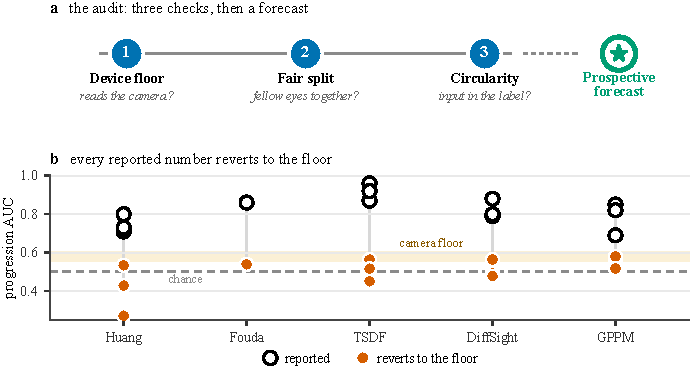
\includegraphics[width=0.9\linewidth]{figures/fig1_audit.pdf}
  \caption{\textbf{The three-check audit, and the floor every published number reverts to.} \textbf{(a)}~A trustworthy
  glaucoma-progression claim should clear three checks that catch shortcuts: a device floor (a model given only the
  acquisition camera), a fair split (fellow eyes kept together), and a circularity check (the input disjoint from the
  window that defines the label). Beyond them is the prospective forecast we prescribe, the baseline visit predicting the
  shipped label. \textbf{(b)}~Every reported number (black, \num{0.71}--\num{0.96}) falls to no better than the camera
  floor (orange, one point per endpoint), where the device, the fellow-eye split, and circularity are controlled
  together, sitting within the shaded floor band ($\approx$\num{0.56}--\num{0.60}, wide enough that the sparse 14-event
  PLR3 can undershoot chance). The per-model reproduce-then-revert behind this teaser is Fig.~\ref{fig:revert}.}
  \label{fig:audit}
\end{figure}

\paragraph{Three shortcut-checks and a prospective test.} The three checks ask whether a high AUC is riding a shortcut,
and a claim passes them only if it clears all three (Fig.~\ref{fig:audit}a). \emph{Check 1
(device floor):} a model given only the acquisition device as input should score at chance. If a device-only model
scores well, the device is confounded with the label and any imaging model can exploit it. (On GRAPE the device is the
camera, so we call this baseline the \emph{camera floor}.) \emph{Check 2 (fair split):} the reported AUC must survive a
fair, patient-grouped, cross-validated evaluation (both eyes of a patient on the same side of every fold, scored across
folds rather than on a single favorable split), or the number is not a reliable estimate of the model. \emph{Check 3 (circularity):} the input must be disjoint from the data window that defines the label. Feeding
the visual fields whose trend defines progression is predicting the label from itself. Beyond these three we prescribe
the positive test a genuine claim should also pass. \emph{The prospective forecast:} predict the shipped label from the
baseline (first) visit, before the trend that defines it is computable. This keeps every event, so it is well powered. A
stricter variant, the strictly-future landmark, predicts only events that fall after the input window. On GRAPE that
leaves too few events to read, so we treat it as a foil, not a main result. Each check uses a field GRAPE already ships:
an acquisition-device label, patient identifiers, the label's definition, and visit timestamps, so any benchmark
carrying these can run all of them (a device-decode probe, a grouped cross-validation, a window-overlap test, and a
baseline-forecast split).

The checks do not carry equal evidential weight on GRAPE. Check 1's device decode uses no outcome labels, Check 2 is a
protocol-level comparison anchored to a training-free floor, and Check 3 reads the continuous visual-field statistics
that define the label. Our main conclusions lean on these three and on the well-powered baseline forecast, not on the
underpowered landmark.

\paragraph{Metrics.} Every AUC we compute is a patient-grouped, repeated five-fold out-of-fold estimate with a patient
cluster-bootstrap 95\% CI \citep{diciccio1996bootstrap}. The eye is the unit, and both eyes of a patient share a fold.
The camera-only floor is the same estimator on a single binary device indicator, no pixels. The device-decoding probe is
a linear classifier that predicts the acquisition device from a frozen RETFound-CFP \citep{zhou2023retfound} embedding,
the feature vector the fundus foundation model extracts from each photograph. The device is controlled with a covariate-adjusted AUC \citep{janes2009aroc}, which conditions the score on the
acquisition device (the binary TOPCON-vs-Canon indicator) so a model cannot use it as a feature. Because the endpoints
carry only 14--40 events, we read intervals, not point estimates. These are descriptive comparisons, not confirmatory
tests.

\paragraph{Cohort.} GRAPE \citep{huang2023grape} has 263 eyes of 144 patients (all glaucomatous, median 4 visits),
with PLR2/PLR3/MD progressors of 40/14/27. Baseline photographs come from three cameras (a TOPCON TRC-NW8 and two
Canon CR-2 models), split 157/106 (TOPCON/Canon) by the dataset's own acquisition-device field. The data are public
(Figshare collection 6406319). Table~\ref{tab:priorclaims} places the five published models against the audit.

\begin{table}[t]
  \centering
  \footnotesize
  \setlength{\tabcolsep}{6pt}
  \renewcommand{\arraystretch}{1.2}
  \caption{\textbf{The published GRAPE progression record against the audit.} Reported AUC is PLR2/PLR3/MD. The
  \emph{Fails} column names the checks the reported number does not clear: a device floor (a model given only the
  acquisition camera), a fair patient-grouped split, and circularity (the input disjoint from the window that defines the
  label). Circularity does not apply to a single baseline image (Huang, Fouda) or two early images (DiffSight, below the
  three-visit slope threshold), which have no serial window to leak. Every reported number fails at least one check, and
  every reported AUC and split is verified from the five source papers (for TSDF, from its released code). $\dagger$:
  weights and key components are unreleased (DiffSight's vessel and optic-disc/cup difference maps, GPPM's evidential
  fusion), so these two are reproduced as a matched model class. Their verdict is that the eye-level protocol inflates
  that class, not a re-run of the exact network.}
  \label{tab:priorclaims}
  \begin{tabular}{@{}lll@{}}
    \toprule
    Model & Reported AUC & Fails \\
    \midrule
    Huang et al.\ \citep{huang2023grape}       & 0.71/0.80/0.73    & device, split \\
    TSDF \citep{song2025tsdf}                   & 0.87/0.96/0.92    & device, split, circularity \\
    DiffSight-Former$^\dagger$ \citep{huang2026diffsight} & 0.79/0.88/0.80 & device, split \\
    GPPM$^\dagger$ \citep{zheng2025gppm}         & 0.85/0.82/0.69    & device, split, circularity \\
    Fouda \& Mohammed \citep{fouda2025}         & 0.86\,(PLR3)      & device, split \\
    \midrule
    \textit{Camera-only floor (ours)}           & 0.561/0.600/0.580 & \textit{reference} \\
    \bottomrule
  \end{tabular}
\end{table}


% ======================================================================================
\section{Findings}
\label{sec:findings}

Each finding makes one claim, with its interval. The four figures trace the audit from shortcut to prospective test.

\begin{figure}[t]
  \centering
  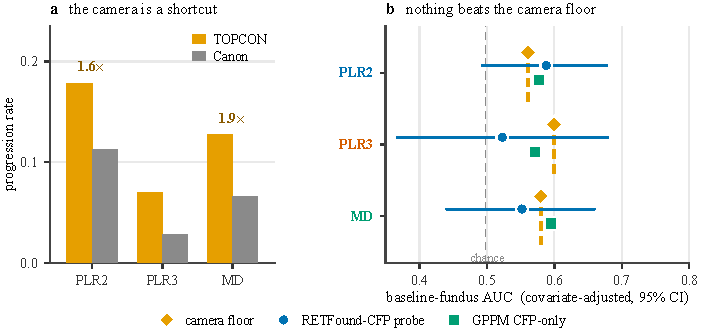
\includegraphics[width=0.9\linewidth]{figures/fig2_device.pdf}
  \caption{\textbf{The device confound and the floor it sets (Check~1, F1).} \textbf{(a)}~The acquisition camera is a
  usable shortcut: TOPCON eyes progress \num{1.6}--\num{1.9}$\times$ as often as Canon (and more often on the sparse
  14-event PLR3 endpoint too), a frozen embedding decodes the camera at out-of-fold AUC \num{0.98}--\num{1.00}, and the camera alone
  (no pixels) predicts progression at \num{0.56}--\num{0.60}. \textbf{(b)}~Every device-controlled estimate of the
  baseline-fundus signal then coincides with that floor (orange): a covariate-adjusted RETFound-CFP probe and GPPM's
  CFP-only baseline. On every endpoint (PLR2/PLR3/MD) no \num{95}\% CI clears the floor.}
  \label{fig:device}
\end{figure}

\paragraph{F1: the acquisition camera is a shortcut, and no representation robustly beats the floor it sets (Check~1).} GRAPE's baseline photographs come from a TOPCON
TRC-NW8 and Canon CR-2 cameras, and the camera is confounded with the label: TOPCON eyes progress \num{1.6}--\num{1.9}$\times$
as often as Canon eyes (Fig.~\ref{fig:device}a). A model given only a
binary TOPCON-vs-Canon indicator (no image content) therefore predicts progression at AUC
\num{0.561}/\num{0.600}/\num{0.580} (Fig.~\ref{fig:device}), a training-free floor that uses no pixels. A frozen
RETFound-CFP embedding distinguishes TOPCON from Canon at out-of-fold AUC \num{0.98}, rising to \num{1.00} on the
optic-disc crop the downstream papers actually use. The device is therefore trivially available to any model, and cropping
does not remove it. The naive fundus-embedding
AUC (\num{0.57}--\num{0.60}) is no higher than the camera floor, and controlling the device (a covariate-adjusted AUC)
leaves it at the floor (Appendix~\ref{app:device}). No published model controls for the device, though the acquisition
field ships with the dataset. The camera does not photograph sicker eyes: baseline severity (visual field, RNFL, IOP) is
matched across cameras, and the confound instead tracks follow-up length (TOPCON eyes are followed longer, so their
slope-defined labels trigger more often), an exposure-time artifact rather than retinal prognosis (App.~\ref{app:device}).

The device-controlled baseline-fundus signal remains near the floor. A frozen RETFound-CFP disc-crop probe (the crop the
downstream papers use), covariate-adjusted for the device, scores \num{0.59}/\num{0.52}/\num{0.55}, the CFP-only baseline of an independent group and architecture
(GPPM's, a generous eye-level upper bound) sits at the floor (App.~\ref{app:setup}), and the
fine-tuned single-CFP models the GRAPE and Fouda papers train are likewise at the floor once the device is controlled
(Fig.~\ref{fig:revert}). A sweep over eight representation-and-crop combinations agrees: every one's interval includes or
sits below the floor, and the one exception (a ConvNeXt-Base probe on MD, \num{0.74}~\ci{0.66}{0.82}) does not replicate
across backbone scale (ConvNeXt-T/B/L give \num{0.49}/\num{0.74}/\num{0.61} on MD) or under fine-tuning
(Table~\ref{tab:ladder}).
No representation we tried clears the floor robustly, so the embedding that identifies the camera at AUC \num{1.00}
carries no baseline-fundus signal we can distinguish from the device. The floor itself carries a wide interval that spans
chance (App.~\ref{app:setup}), so at these event counts these reads are non-inferiority to the floor, not proof that no
fundus signal exists.

\paragraph{F2: the reported range reproduces eye-level, then reverts to the floor (Check~2).} We fine-tuned the
single-CFP architectures the GRAPE and Fouda papers use, with their imbalance recipe (App.~\ref{app:setup}). Under the
standard eye-level split these papers use or imply, the best of our seed runs reaches the published numbers, but those
values sit at the top of a wide seed spread whose medians are
only \num{0.41}--\num{0.70} (Fig.~\ref{fig:revert}): the reported number is the high end, not the center. Under a fair
split the same models revert to \num{0.43}--\num{0.56}, no better than the camera floor. PLR3 is especially fragile: with
14 progressors an eye-level fold holds about three positives, so its AUC takes only a few discrete values, and both the
published \num{0.80} and Fouda's \num{0.86} sit within that seed-to-seed noise. The reversion is not an under-training
artifact: the same recipe reaches the published range eye-level while a frozen probe and a fine-tuned single-CFP model both sit
at the training-free floor (F1), so the drop is the split, not the budget.

\paragraph{The serial-image models reproduce, then revert, on their own code.} TSDF's released code
\citep{song2025tsdf} runs an eye-level \texttt{KFold} and selects the
best epoch on the test fold, a selection-bias inflation of the estimate \citep{cawley2010overfitting}. On its own
released features we recover its numbers to within \num{0.002}
(\num{0.866}/\num{0.954}/\num{0.917}), and fixing three defects (a fair split, held-out epoch selection, and a pooled
out-of-fold AUC) reverts them to \num{0.43}/\num{0.54}/\num{0.55} at the camera floor (Fig.~\ref{fig:revert}). This is a
property of the protocol and of the serial-image class, not one model: a sequence of serial-image variants, from change
features to a temporal attention head, reproduces the reported range eye-level and sits at the patient-grouped floor at
every step (App.~\ref{app:serial}). DiffSight-Former \citep{huang2026diffsight} reports \num{0.79}/\num{0.88}/\num{0.80} on a single
\num{156}/\num{40} eye-level split with two PLR3 test positives. Reproducing its two-image input in its own regime, we
reach those numbers at the eye-level upper tail and drop to the floor (\num{0.49}/\num{0.48}/\num{0.59}) under a fair
split (App.~\ref{app:serial}). Every serial number thus reflects the split rather than the forecast its design intends.

\begin{figure}[t]
  \centering
  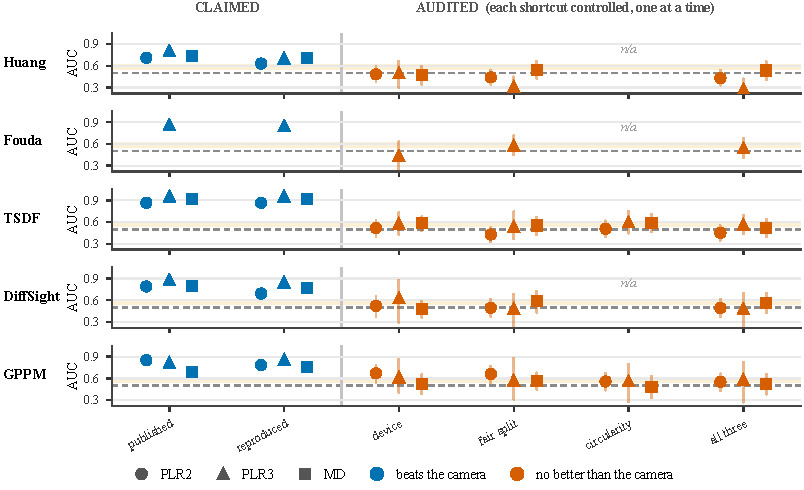
\includegraphics[width=\linewidth]{figures/fig3_revert.pdf}
  \caption{\textbf{Reproduce, then revert: every published number is no better than the camera once each shortcut is
  controlled.} One row per method, reproduced by its own released code or architecture where available (ResNet-50 for
  Huang, a weighted CNN ensemble for Fouda, the released code for TSDF) and by a matched model class where weights are
  unreleased (a two-image change head for DiffSight, GPPM's two-field VF$+$CFP mechanism). For the latter two, the result
  is that the protocol inflates the model class, not that their exact network lacks signal. Each point
  is an endpoint (circle PLR2, triangle PLR3, square MD; PLR3 has only \num{14} events, about three per fold, so its
  single values are noisy). A marker is blue when its \num{95}\% interval clears that endpoint's own camera floor (\emph{beats the camera})
  and orange when the interval includes it (\emph{no better than the camera}). Whiskers are intervals. The
  \textsc{claimed} columns give the published AUC and our reproduction, which recovers it. The \textsc{audited} columns
  control one shortcut at a time, the device (a covariate-adjusted AUC \citep{janes2009aroc}), a fair patient-grouped
  split, and a non-circular input, and then all three together. The four image models are no better than the camera under
  every control. GPPM comes closest: its device- and split-controlled points on PLR2 are the highest of the five (about
  \num{0.67}), but no interval clears the floor, and it reaches the floor once the input is made non-circular.
  \emph{n/a}: the check does not apply, because a single- or two-image input has no serial window to leak.}
  \label{fig:revert}
\end{figure}

\paragraph{F3: the circularity dial (Check~3).}
The progression labels are a trend fit to an eye's visual-field series, so feeding that series to predict the label is
predicting the label from itself. Circular analysis warns that using the same data to define and to estimate a quantity
distorts it whenever the two are not independent \citep{kriegeskorte2009circular}. Here the quantity is the label and the
data are the visual fields. We turn that warning into a measurement. A \emph{circularity dial} tracks the leakage as the
input window lengthens toward the window that defines the label (Fig.~\ref{fig:circular}a): predicting the fixed MD label
from the visual-field statistics of the first $k$ visits climbs from \num{0.47} at one visit to
\num{0.90} once the whole series is available, and the jump lands exactly at $k{=}3$, when a slope and its $p$-value
first become computable. That threshold is sharp: a slope and its $p$-value cannot be computed from fewer than three
visits (two points give a slope but no significance), so an input spanning one or two visits cannot recover the
label-defining statistic and stays near chance. The onset is a property of the label, not of counting visits:
loosening the slope's significance threshold ($p<0.10$) leaves the jump at $k{=}3$, while a placebo label defined by a
two-visit change (computable at $k{=}2$) has its jump at $k{=}2$ instead (App.~\ref{app:dialrobust}). A two-field pair
lifts the score by a separate, weaker route. The pair recovers the label only when the second field falls inside the
label-defining window, so it is the time span that leaks, not the slope (Fig.~\ref{fig:circular}b). A statistic
ablation confirms the mechanism: the label-defining slope (AUC \num{0.91}) and its
$p$-value (\num{0.95}) carry the \num{0.90}, while recency, variability, and visit count do not (Fig.~\ref{fig:circular}c).
The dial is general: any benchmark whose label is a trend fit to a series can be probed the same way, providing a direct
test for a familiar pattern. Progression AUCs often rise with the number of input visits, and this is usually read as a model
accumulating evidence. Read this way, the rise is instead leakage accruing as the input window grows into the
label-defining window. It affects any model whose input reaches into that window, and most directly a
visual-field-history model, which reads the defining statistics themselves.

GPPM's fusion is the clearest instance, and we reproduce its mechanism on GRAPE. It pairs a
baseline visual-field test with one follow-up test (its fundus branch is down-weighted to \num{0.01}, so the visual
field carries the number), and a two-field pair recovers the fixed label only when the second test is late: the
baseline-and-last pair scores \num{0.83}/\num{0.86}/\num{0.86}, while a baseline-and-second pair (both fields early,
before the label window) sits at chance (\num{0.51}--\num{0.53}). Sweeping the second test later lifts the AUC with its time span,
not the count of two (Fig.~\ref{fig:circular}b). This is about what GPPM's input carries, not its architecture: its own
fundus-only branch already sits at the camera floor (App.~\ref{app:setup}), so the fusion's lift is in-window field
change, not baseline prognosis, and the same early pair forecasts a strictly later event no better than chance. The
serial-fundus models are a
weaker, less clear-cut case. TSDF consumes the full fundus visit sequence, which
reaches into the same window, so its lift is at least partly structural change occurring during that window rather than
a prospective forecast (App.~\ref{app:serial}). DiffSight-Former frames its task as forecasting future onset, a claim
GRAPE's short series cannot adjudicate.

\paragraph{The prospective forecast we prescribe stays at the floor.} The positive test that no paper runs is to predict the
shipped label from the baseline visit, before the trend that defines it is computable. This forecast is
non-circular and keeps the full event counts (\num{40}/\num{14}/\num{27}), so it is
well powered on the PLR2 and MD arms. On GRAPE it cannot beat the camera floor: the baseline fundus sits at the floor
(\num{0.60}/\num{0.57}/\num{0.59}), and a multimodal fusion of the visual field, optical coherence tomography (OCT),
fundus, and intraocular pressure (IOP) is no better (App.~\ref{app:serial}). The baseline forecast is thus at the floor
even as the circular in-window number reaches \num{0.90}, so GRAPE places progression at the floor while it stays
forecastable at scale (\S\ref{sec:discussion}).

\begin{figure}[t]
  \centering
  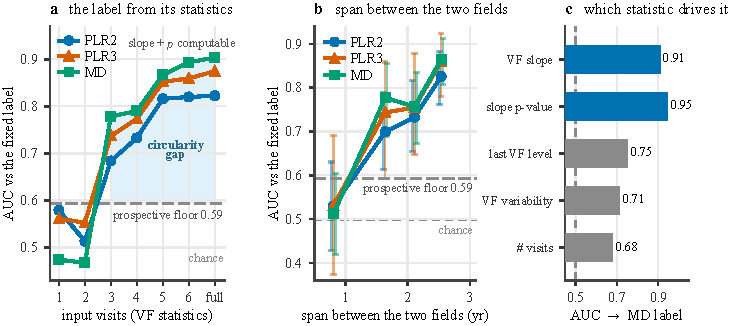
\includegraphics[width=\linewidth]{figures/fig4_circular.pdf}
  \caption{\textbf{The \num{0.90} comes from predicting the label from its own statistics (Check~3).} \textbf{(a)}~Out-of-fold
  AUC for predicting the fixed label GRAPE provides from the visual-field statistics of the first $k$ visits, as $k$ grows
  into the window that defines the label. The MD AUC climbs \num{0.47}$\rightarrow$\num{0.90}, jumping once the slope and
  its $p$-value become computable ($k{=}3$). The baseline prospective forecast (first visit $\rightarrow$ the shipped
  label, dashed) sits at the camera floor ($\approx$\num{0.59}, on the full event counts \num{40}/\num{14}/\num{27}), and
  the shaded band between it and the circular curves is the circularity gap.
  \textbf{(b)}~The two-field model (GPPM's mechanism): a pair of visual-field tests recovers the fixed label only when the
  second test is late. As the span between the two tests grows (baseline$+$2nd $\rightarrow$ baseline$+$last), the AUC
  climbs from chance to \num{0.86} (95\% CI whiskers), so it is the span that leaks, not the count of two. The early
  pre-window pair sits at chance, and the baseline prospective forecast (dashed) stays at the floor. \textbf{(c)}~Full-series AUC from each statistic alone: the label-defining slope (\num{0.91}) and its
  $p$-value (\num{0.95}) carry the \num{0.90}, not recency, variability, or visit count.}
  \label{fig:circular}
\end{figure}

% ======================================================================================
\section{Discussion and limitations}
\label{sec:discussion}

\paragraph{What this means for the field.} We read these as failures of the evaluation setup, not of the teams behind
these models. The confound comes from scoring a device-confounded,
visual-field-labeled public benchmark by a single leaderboard AUC, a pitfall the shortcut-learning literature documents
across medical imaging \citep{geirhos2020, zech2018}. To the resolution the data allow, the published numbers are
protocol artifacts: a device shortcut, an eye-level split, and label circularity account for the reported range where we
reproduce it (Fig.~\ref{fig:revert}), and no estimate we tried clears the floor.
This does not say progression is unpredictable: in large, device-controlled cohorts baseline models forecast trajectory
progression at AUC \num{0.84} (\num{0.75} on an external device) \citep{mohammadzadeh2026} and glaucoma \emph{onset} at
$\approx$\num{0.74} \citep{ohts2007validated}. But GRAPE, at 14--40 events with a device-confounded, VF-derived label,
cannot establish it: its numbers measure the protocol, not the eye.

\paragraph{What to do instead.} The audit suggests one practical fix for each check. For the device, report the camera
floor and a covariate-adjusted AUC. For a fair split, keep each patient's two eyes on the same side of a cross-validated
split. For circularity, keep the model input disjoint from the label-defining window. And report a baseline prospective
forecast, the first visit predicting the label, alongside any in-window number, each with a cluster-bootstrap interval
at the stated event count. These changes make a leaderboard number easier to interpret as a clinical claim. We release a
fixed patient-grouped split and a reporting template so the protocol can be applied consistently
(App.~\ref{app:template}).

\paragraph{Limitations.} \emph{Small event counts.} With 14--40 events the per-endpoint intervals are wide. We lean on
the event-independent device decode, the training-free floor and split comparison, and the well-powered PLR2 and MD
arms, and corroborate the floor with several estimates rather than one. \emph{A single cohort.} GRAPE is one
all-glaucoma dataset. The audit is cohort-agnostic, an independent group's CFP-only baseline already reproduces our
floor \citep{zheng2025gppm}, and the mechanisms it exposes (device shortcut, fellow-eye leakage, label circularity) are
established in the ML literature \citep{geirhos2020, kapoor2023leakage}, so running the audit on a second
multi-site cohort is the natural validation and future work. \emph{VF-derived labels.} Every GRAPE label is a
visual-field trend. That circularity is one of our findings (F3) but also precludes a genuine structural endpoint here.
\emph{Serial reproduction.} We reproduce TSDF on its released code and DiffSight as a matched model class (its weights
are unreleased) on GRAPE's short image sequence. Both revert to the floor (App.~\ref{app:serial}).

% ======================================================================================
\section{Conclusion}
\label{sec:conclusion}

A glaucoma-progression AUC on GRAPE can be high because a model reads the camera, because a patient's two eyes leak
across the split, or because the input already contains the label, and none of these is visible to a single-split AUC.
Our audit makes these sources visible with three checks, a device floor, a fair split, and a circularity dial that
reads the label leaking back into the input as the window grows, and adds a baseline prospective forecast for the
prediction that would actually count. Applied to GRAPE, every published
progression number fails at least one check, and the baseline-fundus signal cannot, at this sample size, be
distinguished from a training-free camera floor (\num{0.56}--\num{0.60} across endpoints). On GRAPE today, a high score
can still come from the camera, the split, or the label. Until a number clears all three checks and also forecasts a
held-out future, it is not yet evidence about the eye.
